\documentclass[11pt,english,a4paper,twoside]{article}
%\documentclass[11pt,slovak,a4paper,twoside]{article}

\usepackage[IL2]{fontenc}
\usepackage[utf8]{inputenc}
\usepackage{babel}
\usepackage{url}
\usepackage[nottoc]{tocbibind}
\usepackage{ifthen}
\usepackage[hidelinks]{hyperref}
\usepackage{graphicx}
\usepackage{listings}
\usepackage{float}

\raggedbottom
\oddsidemargin=0cm
\evensidemargin=0cm
\textwidth=16.5cm
\pagestyle{plain}

\newcommand{\reporttitle}{AASS Semestral project}

\title{\reporttitle}

\author{
        Lukáš Častven, Michal Kilian\\[2pt]
	{\small Slovenská technická univerzita v Bratislave}\\
	{\small Fakulta informatiky a informačných technológií}\\
	{\small \texttt{xcastven@stuba.sk, xkilian@stuba.sk}}
}

\date{\today}
\begin{document}
\maketitle

\section{Application overview}

The name of our application is Healendar (heal + calendar). 

\section{Stakeholders}

\begin{table}[h!]
  \centering
  \begin{tabular}{|p{0.25\linewidth}|p{0.5\linewidth}|}
    \hline
    \textbf{Stakeholder} & \textbf{Description} \\
    \hline
    Patient & Wants to book appointment with doctor. \\
    \hline
    Nurse & Accepts or rejects appointment requests,
    requests more information from patients, and selects
    specialized rooms. \\
    \hline
    Doctor & Needs to see their workload and can override
    nurse decisions regarding appointments. \\
    \hline
    Other hospital staff & Needs to see the availability of
    other doctors and specialized rooms for their patients. \\
    \hline
    Hospital & Desires a new application to organize
    doctors and appointments. \\
    \hline
  \end{tabular}
  \caption{Stakeholders and Their Descriptions}
  \label{tab:stakeholders}
\end{table}

\section{Motivation}

The following motivation diagram contains the drivers, assessments, goals,
outcomes, and requirements related to the 4 identified stakeholders.
Patient, Hospital, Nurse, Doctor.

The core problems, "High operational costs", "Long waiting times", and a "Bad
reputation for possible new hires", drive the hospital for change. These drivers
are associated with issues such as "Ineffective allocation", "Medical
staff frustration", "Unavailability of specialized rooms",
and patients' "Waiting times."

\pagebreak
\begin{figure}[ht]
    \centering
    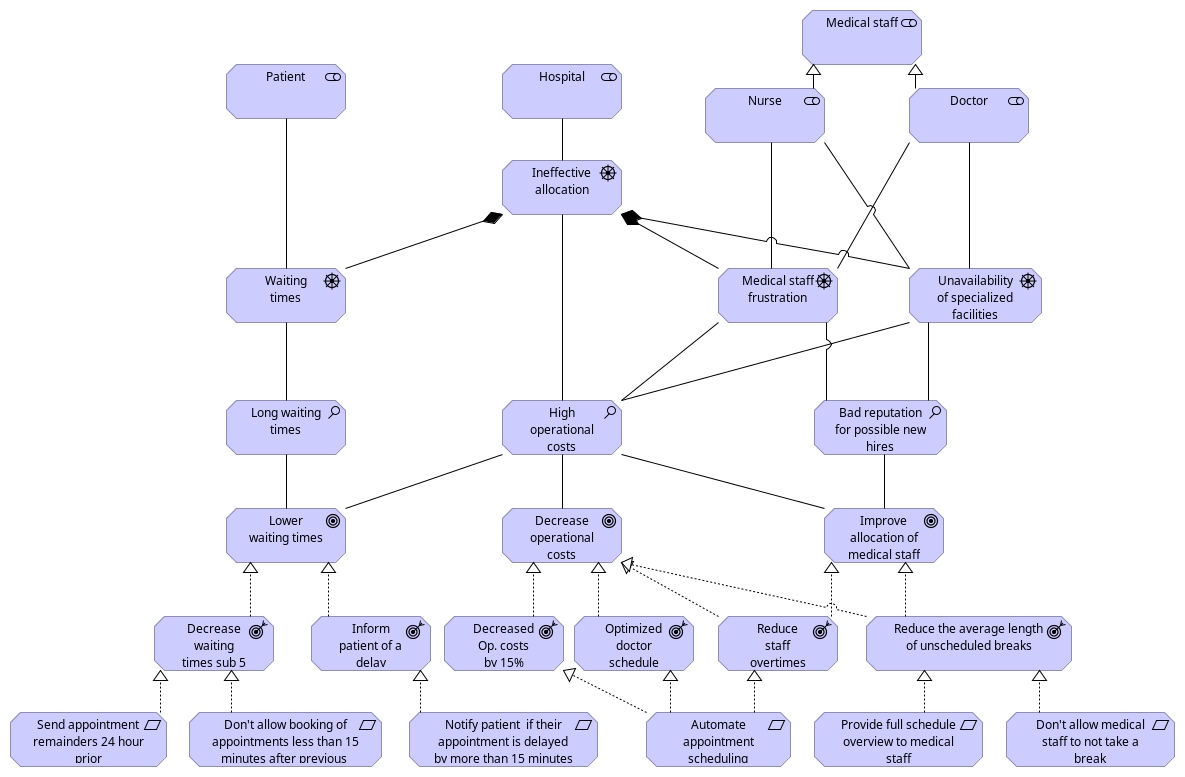
\includegraphics[width=\textwidth]{./fig/Motivation.png}
    \caption{Motivation layer of Healendar}
    \label{fig:motivation}
\end{figure}

\pagebreak
\section{Value stream}

The value stream of scheduling an appointment realizes the outcome of optimized
doctor schedule.

\begin{figure}[ht]
    \centering
    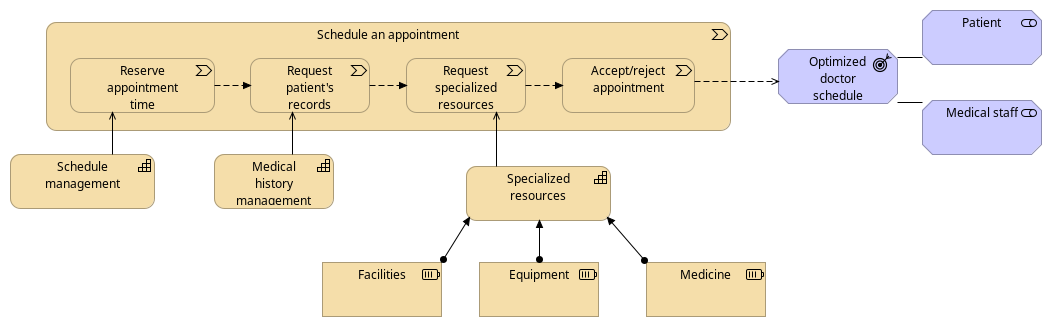
\includegraphics[width=\textwidth]{./fig/Value stream.png}
    \caption{Value stream: Scheduling appointment}
    \label{fig:value_stream}
\end{figure}

\pagebreak
\section{Business layer}

Following diagram models three business processes, which serve the patient
and medical staff to manage schedule.

\begin{figure}[ht]
    \centering
    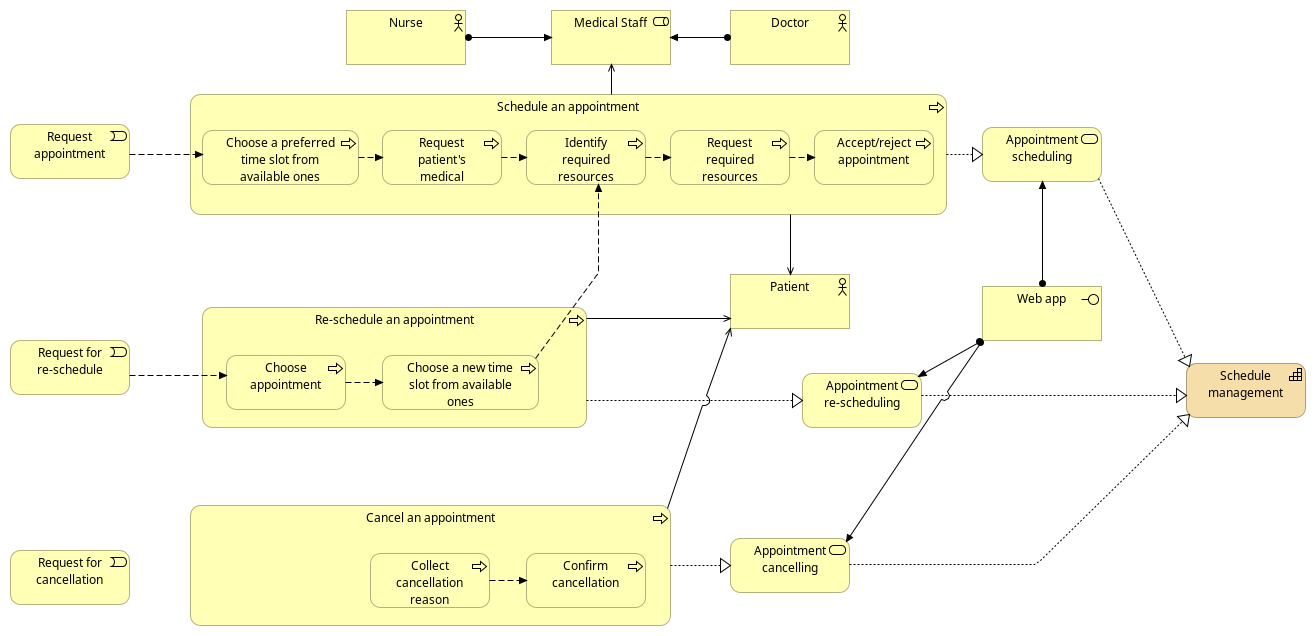
\includegraphics[width=\textwidth]{./fig/Business.png}
    \caption{Business layer}
    \label{fig:business}
\end{figure}

\section{Mockups}

The patient interface, Figure~\ref{fig:patient-mockups}, shows
a design centered on appointment scheduling.
Figure~\ref{fig:medical-staff-mockups} illustrates the UI for the
same use case, but with more control and additional resources requests
for the medical staff.

\begin{figure}[H]
    \centering
    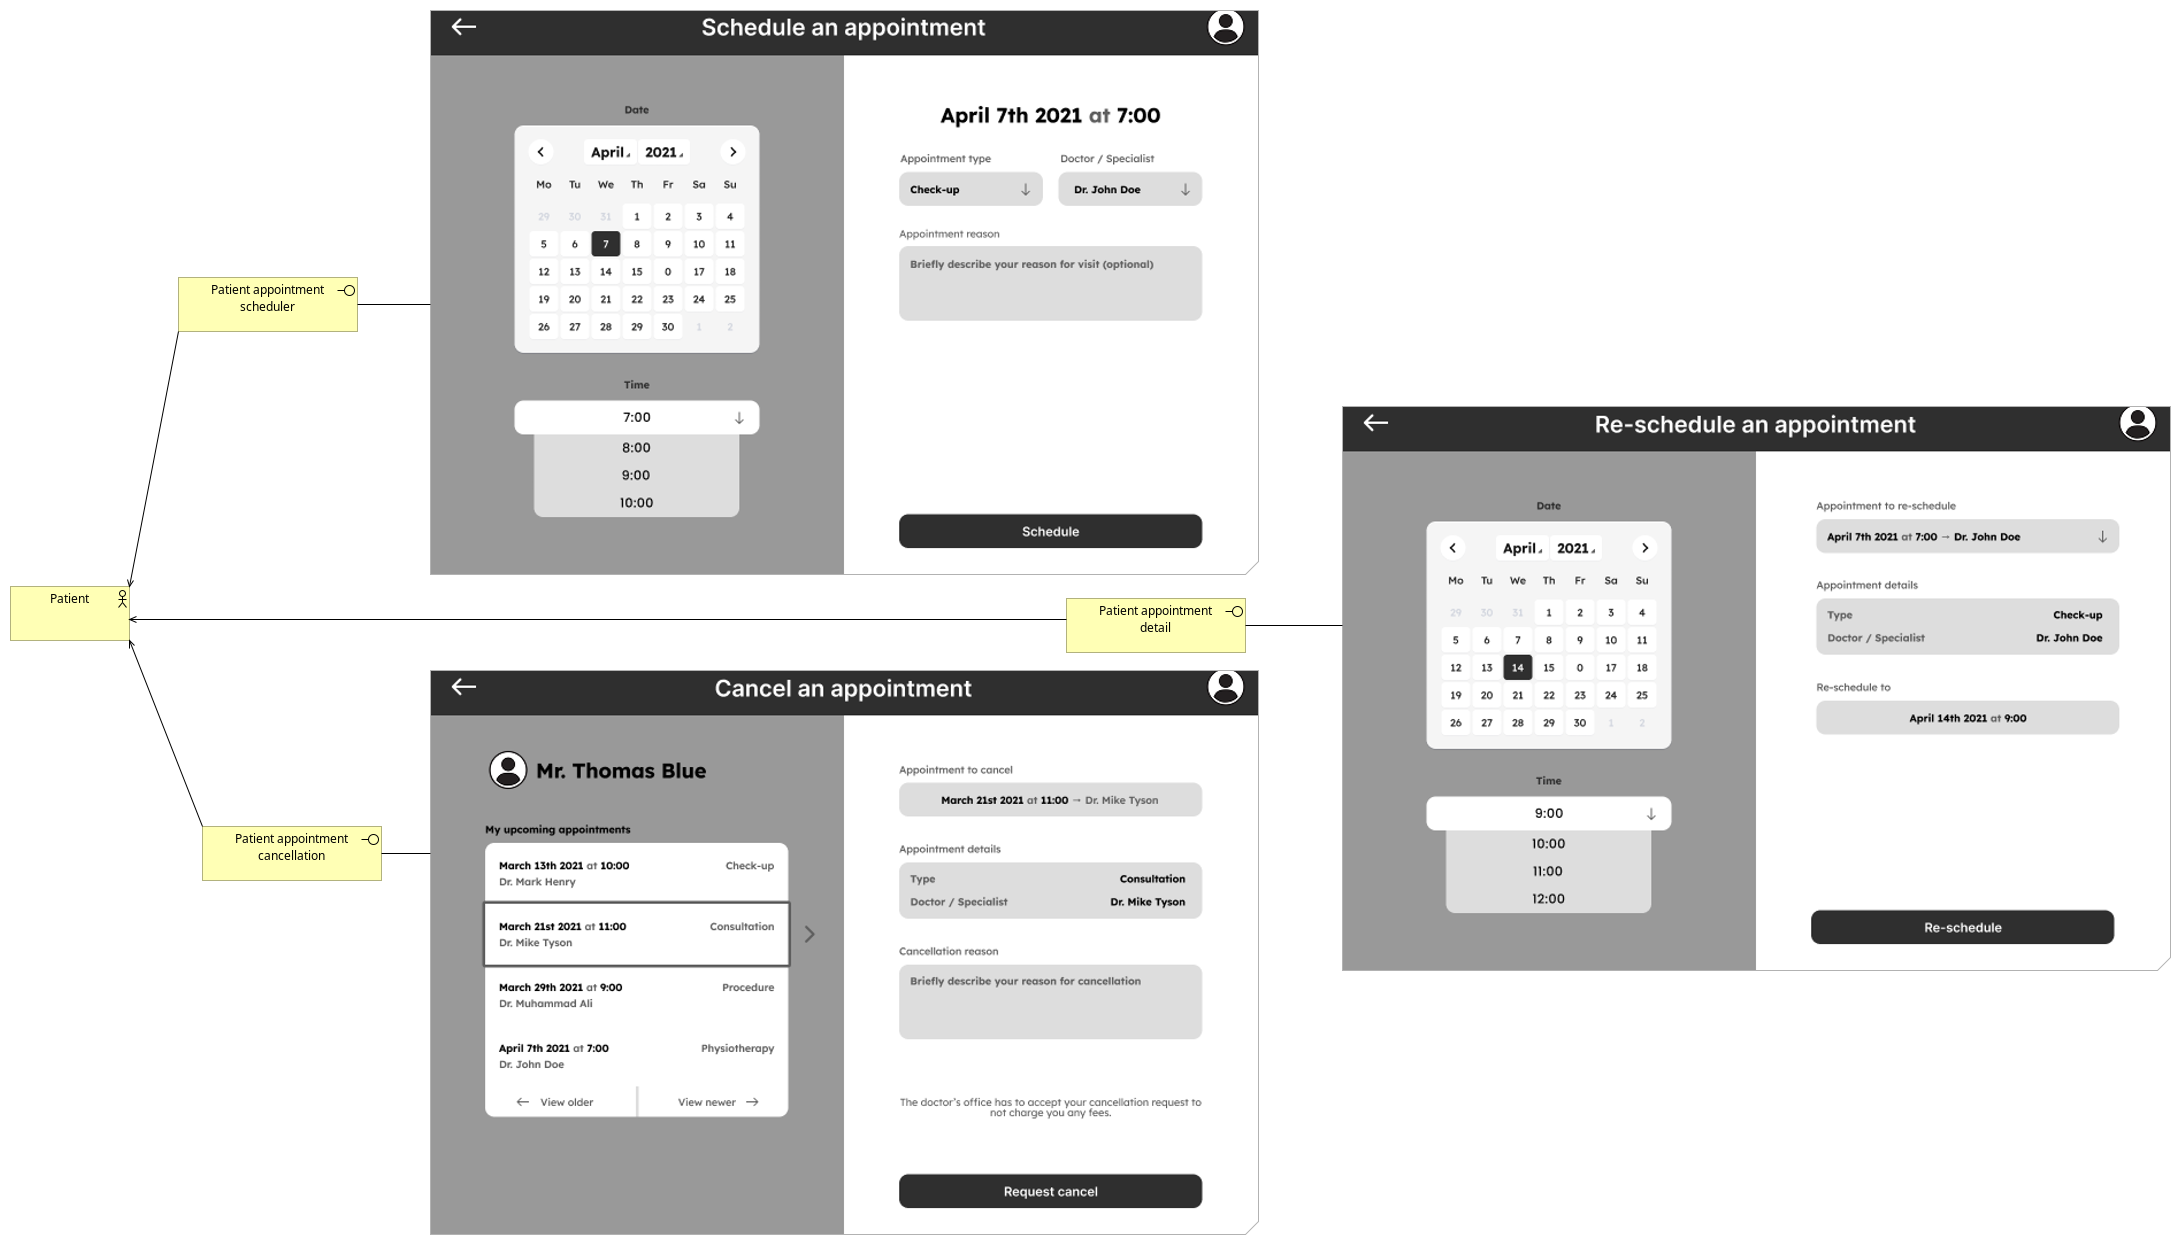
\includegraphics[width=\textwidth]{./fig/Business Frontend Patient.png}
    \caption{Patient's UI mockups}
    \label{fig:patient-mockups}
\end{figure}

\begin{figure}[H]
    \centering
    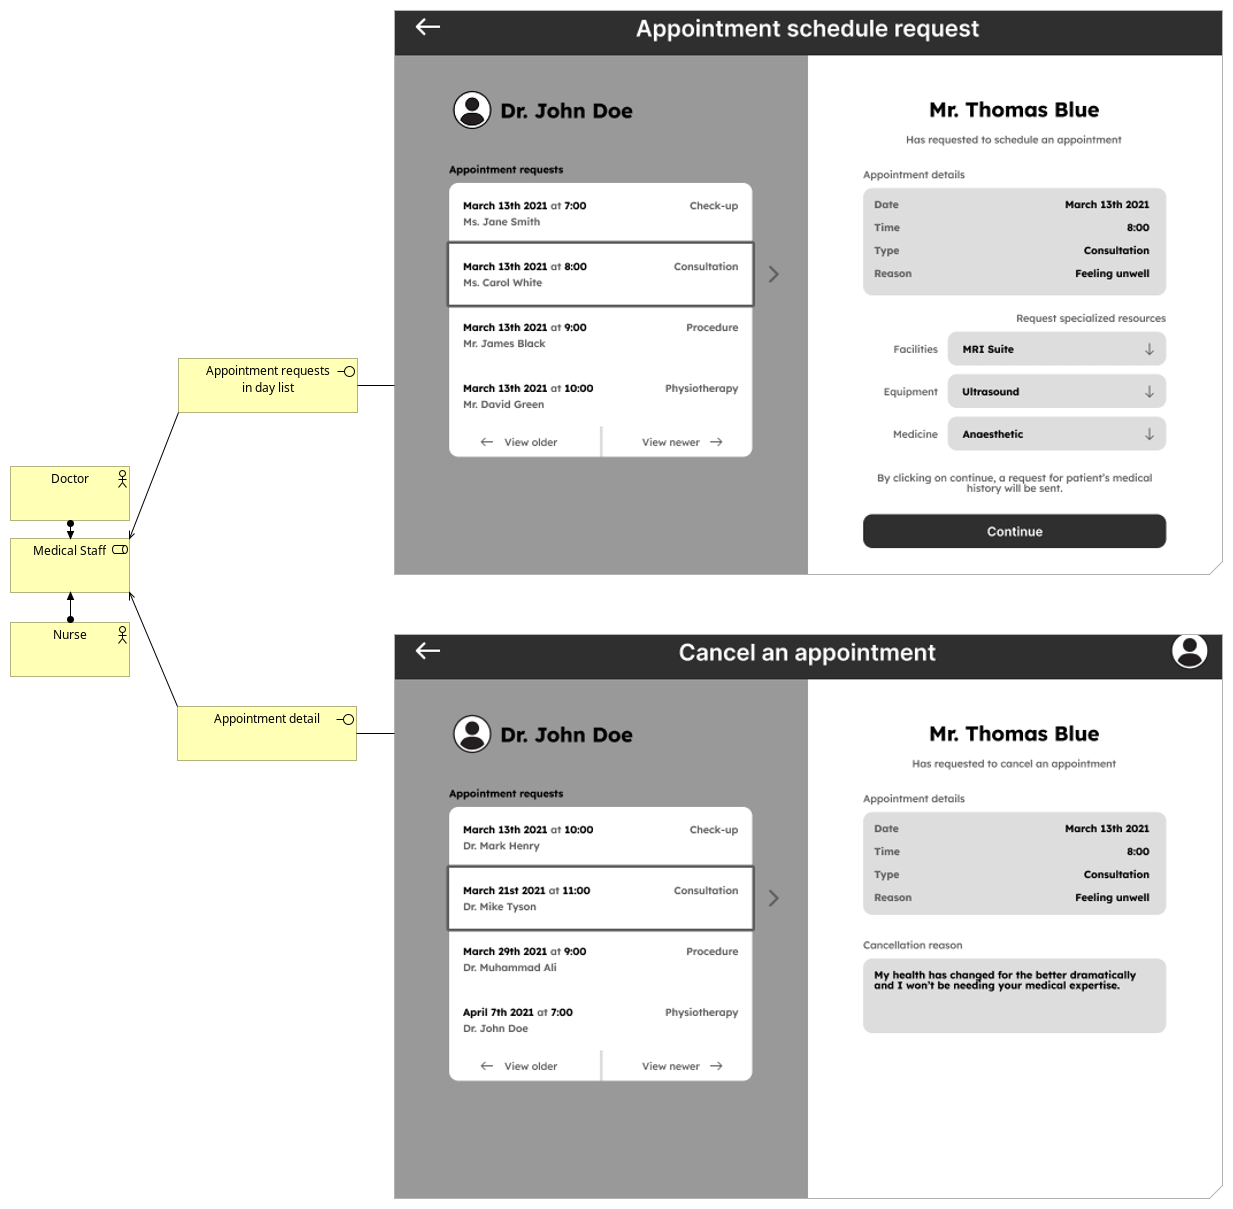
\includegraphics[width=\textwidth]{./fig/Business Frontend Medical staff.png}
    \caption{Medical staff's UI mockups}
    \label{fig:medical-staff-mockups}
\end{figure}

\section{Architecture 1 application layer}

We will implement a user interface and a backend components to
support the "Schedule an appointment" business process. The implementation
will consist of a monolithic backend written in Go and a web application
frontend developed using Stencil.js.

\begin{figure}[H]
    \centering
    \includegraphics[width=\textwidth]{./fig/Application.png}
    \caption{Application layer architecture supporting appointment scheduling}
    \label{fig:application-layer}
\end{figure}
%\bibliography{bibliography}
%\bibliographystyle{ieeetr}

\end{document}
